\documentclass[11pt]{article}

\usepackage[utf8]{inputenc}
\usepackage[T1]{fontenc}
\usepackage[margin=1in]{geometry}
\usepackage{amsmath, amssymb}
\usepackage{graphicx}
\usepackage{booktabs}
\usepackage{float}
\usepackage{caption}
\usepackage{xcolor}
\usepackage{fancyhdr}
\usepackage{hyperref}

\graphicspath{{figures/}}
\captionsetup{font=small, labelfont=bf}

\pagestyle{fancy}
\fancyhf{}
\lhead{AA 274A -- Homework 1}
\rhead{Auguste Vanier (avanier)}
\cfoot{\thepage}

% ---------------------------------------------------------------------------
% Placeholders: replace the \todo{...} inside each environment with your text.
% ---------------------------------------------------------------------------
\newcommand{\todo}[1]{\textcolor{red}{\textit{[#1]}}}

% Space for a written answer
\newenvironment{answer}
  {\par\medskip\noindent\textbf{Answer.}\ }
  {\par\medskip}

% Space for a comment on a figure or table
\newenvironment{figcomment}
  {\par\smallskip\noindent\textbf{Comment.}\ }
  {\par\medskip}

\newcommand{\Lone}{\mathcal{L}^1}
\newcommand{\Ltwo}{\mathcal{L}^2}
\newcommand{\Linf}{\mathcal{L}^\infty}

\title{AA 274A: Principles of Robot Autonomy I \\ Homework 1}
\author{Auguste Vanier \\ SUNet ID: \texttt{avanier}}
\date{October 8, 2026}

\begin{document}
\maketitle

\noindent\textbf{Collaborators: None} 

\medskip
\noindent\textbf{Use of generative AI:To generate the full LateX template but every comments were written by myself. I also used AI to help me figured out the mistakes that were at the origin of code errors}

% ===========================================================================
\section*{Problem 1: A* Motion Planning \& Path Smoothing}
% ===========================================================================

\subsection*{(i) A* implementation}

\begin{figure}[H]
  \centering
  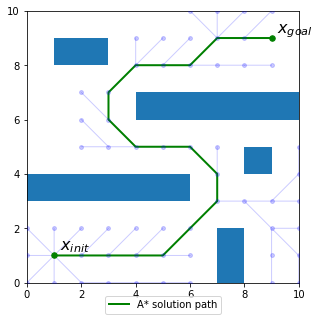
\includegraphics[width=0.6\textwidth]{p1_astar_simple.png}
  \caption{A* path in the simple environment.}
  \label{fig:p1-simple}
\end{figure}

\begin{figcomment}
  The path that was found is the shortest one with this mesh
\end{figcomment}

\begin{figure}[H]
  \centering
  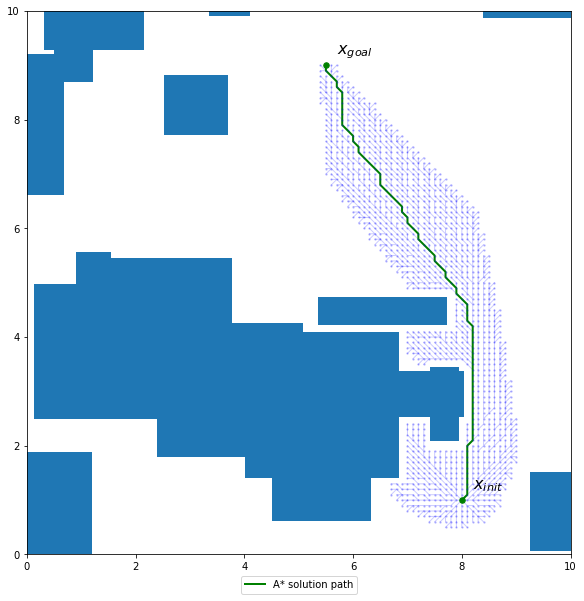
\includegraphics[width=0.6\textwidth]{p1_astar_cluttered.png}
  \caption{A* path in the random cluttered environment (default parameters, \texttt{SEED = 274}).}
  \label{fig:p1-cluttered}
\end{figure}

\begin{figcomment}
  We can see that the whole mesh was not explored but the path seems to be the fastest too
\end{figcomment}

\subsection*{(ii) Path smoothing}

\begin{figure}[H]
  \centering
  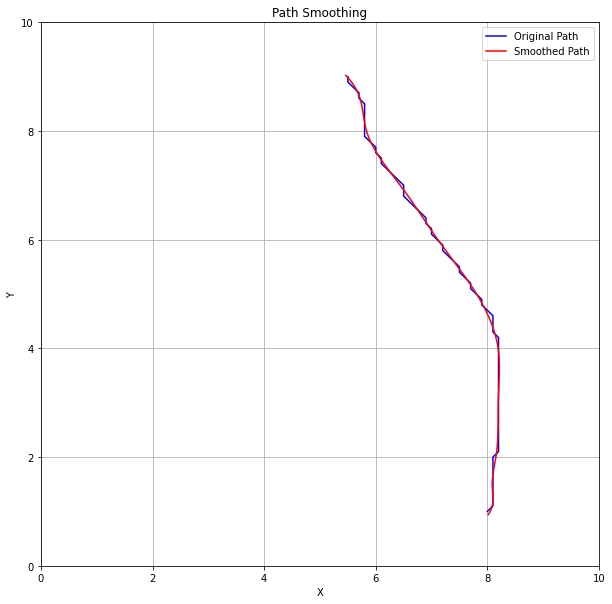
\includegraphics[width=0.6\textwidth]{p1_smooth_trajectory.png}
  \caption{A* path and cubic-spline smoothed path in the random cluttered environment ($v_{des} = 0.15$~m/s).}
  \label{fig:p1-smooth}
\end{figure}

\begin{figcomment}
  This figure shows well how the smoothed path helps to have a better trajectory while being even shorter in this case
\end{figcomment}

\paragraph{Chosen smoothing parameter.}
% The notebook currently calls compute_smooth_plan with its default spline_alpha=0.05.
$\alpha = $ 0.1

\paragraph{Effect of a very large $\alpha$.}
\begin{answer}
  As $\alpha$ grows, the deviation of the spline from the nodes is greater. In fact, the bigger the smoothness is the greater it allows to cut corners or miss points. Therefore, you could miss the start point, miss the goal point or even hit obstacles as no collision program is ran. 
\end{answer}

\subsection*{(iii) Heuristic comparison}

\begin{figure}[H]
  \centering
  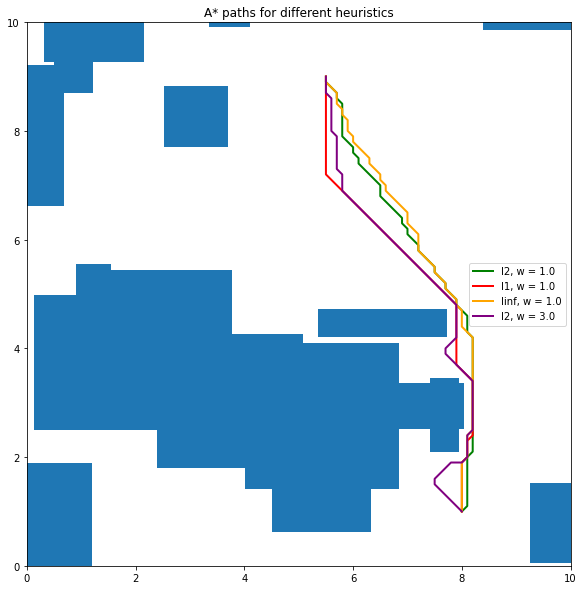
\includegraphics[width=0.9\textwidth]{p1_heuristic_comparison.png}
  \caption{Heuristic comparison on the random cluttered environment (\texttt{SEED = 274}).}
  \label{fig:p1-heuristics}
\end{figure}

\begin{table}[H]
  \centering
  \caption{Path length and number of nodes expanded for each heuristic.}
  \label{tab:p1-heuristics}
  \begin{tabular}{lccc}
    \toprule
    Heuristic & $w$ & Path length & Nodes expanded \\
    \midrule
    $\Ltwo$ & 1.0 & 9.201 & 1091 \\
    $\Lone$ & 1.0 & 9.201 & 318  \\
    $\Linf$ & 1.0 & 9.201 & 1965 \\
    $\Ltwo$ & 3.0 & 9.898 & 146  \\
    \bottomrule
  \end{tabular}
\end{table}

\begin{figcomment}
  The Table shows that with less Nodes the $\Lone$ heuristic with $w=1$ has the best path where the $\Ltwo$ with $w=3$ has the longest path but with only 146 Nodes expanded !
\end{figcomment}

\subsubsection*{(a) Admissibility of the $\Ltwo$, $\Lone$ and $\Linf$ heuristics ($w = 1$)}
\begin{answer}
  We are in an 8-connected grid.

  \medskip\noindent\textbf{$\Lone$:} for the vector $u = (1, 1)$, $\|u\|_1 = 2$ but the real distance is $\sqrt{2}$, so $\Lone$ is not admissible.

  \medskip\noindent\textbf{$\Ltwo$:} let's take the distance between points $i$ and $i+1$. We have
  \[
    c(x_i, x_{i+1}) \geq \|x_{i+1} - x_i\|_2 .
  \]
  Let's sum over $n$:
  \[
    C^*(x) = \sum_{i=1}^{n} c(x_i, x_{i+1}) \geq \sum_{i=1}^{n} \|x_{i+1} - x_i\|_2 \geq \|x_{goal} - x\|_2 = h_2(x)
  \]
  by the triangular inequality. Therefore $C^*(x) \geq h_2(x)$.

  \medskip\noindent\textbf{$\Linf$:} moreover, let $x \in \mathbb{R}^n$. There exists $i \in [\![1, n]\!]$ such that $|x_i|^2 = \max_i (x_i)^2$, and $\sum_{i=1}^{n} |x_i|^2 \geq |x_i|^2$, so
  \[
    \sum_{i=1}^{n} |x_i|^2 \geq \max_i (x_i)^2 .
  \]
  We can take the root of this inequality because the root function is increasing and positive, so
  \[
    \|x\|_2 \geq \|x\|_\infty \iff h_2(x) \geq h_\infty(x) .
  \]
  Therefore $C^*(x) \geq h_2(x) \geq h_\infty(x)$, and $\Ltwo$ and $\Linf$ are admissible.
\end{answer}

\subsubsection*{(b) Ordering of the number of nodes expanded}
\begin{answer}
  From (a), $h_\infty(x) \leq h_2(x)$, and in the same way $h_2(x) \leq h_1(x)$, so the number of nodes expanded is ordered as $\Lone$ ($318$) $< \Ltwo$ ($1091$) $< \Linf$ ($1965$).
  Because as the heuristic is closer to the true length, it goes further every time, so fewer expansions are needed.
\end{answer}

\subsubsection*{(c) Weighted A* and suboptimality bounds}
\begin{answer}
  We know that
  \begin{align*}
    & \|x\|_2 \leq C^*(x) \leq \|x\|_1 \leq \sqrt{2}\, \|x\|_2 \\
    \iff\ & \frac{1}{\sqrt{2}}\, C^*(x) \leq \frac{\|x\|_1}{\sqrt{2}} \leq \|x\|_2 \\
    \iff\ & \frac{C^*(x)}{\sqrt{2}} \leq \frac{\|x\|_1}{\sqrt{2}} \leq C^*(x) .
  \end{align*}
  Therefore, $\dfrac{\|x\|_1}{\sqrt{2}}$ is admissible. The $\Lone$ heuristic is thus an admissible heuristic weighted by $w = \sqrt{2}$, so its path is at most $\sqrt{2}$ times the optimal length, which is consistent with the table ($9.201$ is the optimal length).

  \medskip\noindent For $\Ltwo$ with $w = 1$ and $w = 3$:
  \[
    \mathrm{err} = \frac{\mathrm{length}_3 - \mathrm{length}_1}{\mathrm{length}_1} = 7.6\% \leq 200\% ,
  \]
  and $\Ltwo$ ($w = 1$) uses $7.5\times$ the number of nodes expanded by $\Ltwo$ ($w = 3$) because of the weight.
\end{answer}

% ===========================================================================
\section*{Problem 2: Rapidly-exploring Random Trees (RRT)}
% ===========================================================================

\subsection*{(i) Geometric RRT}

\begin{figure}[H]
  \centering
  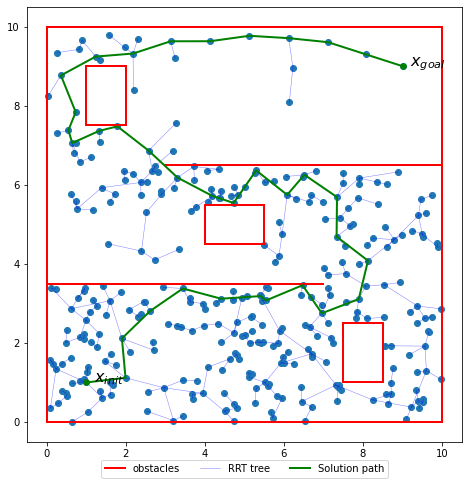
\includegraphics[width=0.6\textwidth]{p2_rrt_geometric.png}
  \caption{Geometric RRT tree and solution path (default start and goal, \texttt{SEED = 274}).}
  \label{fig:p2-rrt}
\end{figure}

\begin{figcomment}
  This path is good but not optimal.
\end{figcomment}

\subsection*{(ii) Shortcutting}

\begin{figure}[H]
  \centering
  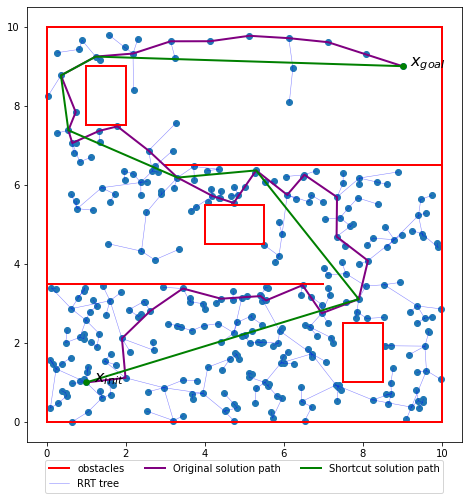
\includegraphics[width=0.6\textwidth]{p2_rrt_shortcut.png}
  \caption{Geometric RRT solution path before and after shortcutting.}
  \label{fig:p2-shortcut}
\end{figure}

\begin{figcomment}
  The shortcuttting helps to get a shorter path, it would be interested to use the smoothing algorithm on it !
\end{figcomment}

\subsection*{(iii) Goal-bias experiment}

\begin{figure}[H]
  \centering
  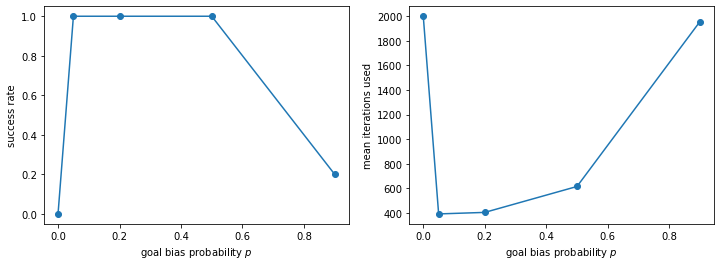
\includegraphics[width=0.95\textwidth]{p2_goal_bias.png}
  \caption{Success rate and mean number of iterations over 20 RRT runs for each goal-bias probability $p$.}
  \label{fig:p2-goal-bias}
\end{figure}

\begin{table}[H]
  \centering
  \caption{Goal-bias experiment results (20 trials per value of $p$, at most 2000 iterations).}
  \label{tab:p2-goal-bias}
  \begin{tabular}{ccc}
    \toprule
    Goal bias $p$ & Success rate & Mean iterations \\
    \midrule
    0.00 & 0.00 & 2000.0 \\
    0.05 & 1.00 & 391.9 \\
    0.20 & 1.00 & 404.2 \\
    0.50 & 1.00 & 615.1 \\
    0.90 & 0.20 & 1956.7 \\
    \bottomrule
  \end{tabular}
\end{table}

\begin{figcomment}
  The best value of p seems to be near 0.05
\end{figcomment}

\subsubsection*{(a) Why RRT essentially never succeeds when $p = 0$}
\begin{answer}
  For $p = 0$, RRT never succeeds because no direction is prioritiazed so it is very unlikely that the path will be created with randomness.
\end{answer}

\subsubsection*{(b) Why the success rate drops again for large $p$}
\begin{answer}
  If you reach 1, the success rate will also drop to zero has the only direction available would be the one between the initial point and the goal point. With $p=0.9$, the probability of other directions is very low which could explain the 0.2 Success rate !
\end{answer}

% ===========================================================================
\section*{Problem 3: Heading Controller}
% ===========================================================================

\subsection*{7. Heading controller response}

\begin{figure}[H]
  \centering
  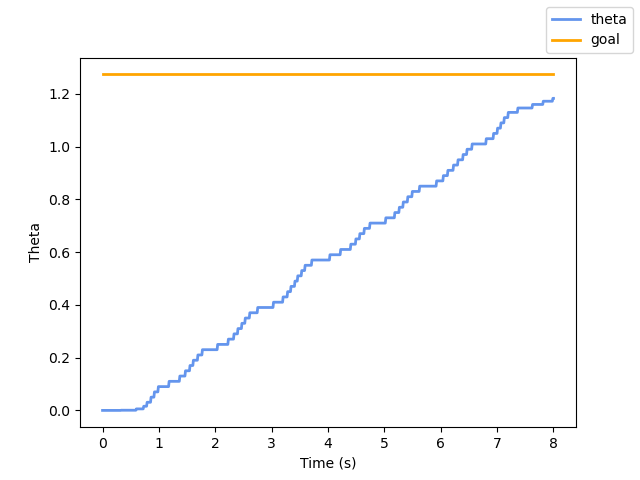
\includegraphics[width=0.7\textwidth]{p3_output.png}
  \caption{Heading $\theta$ of the TurtleBot under proportional control ($k_p = 2$) for the goal heading $\theta_{goal} = 1.274$~rad.}
  \label{fig:p3-output}
\end{figure}

\begin{figcomment}
  The plotting is strange, it is more like a straight line rather than an exponetial function
\end{figcomment}

\subsection*{8. Effect of the gain $k_p$ on the closed-loop behavior}

\subsubsection*{(a) Continuous-time error dynamics}
\begin{answer}
  We have
  \[
    \dot{\theta} = \omega = k_p (\theta_{goal} - \theta) = k_p e ,
  \]
  with $e$ the error and $e = \theta_{goal} - \theta$. But $\dot{e} = -\dot{\theta}$, so
  \[
    \dot{e} + k_p e = 0 .
  \]
  Therefore, $\forall t \geq 0$, $e(t) = e_0\, e^{-k_p t}$.

  \medskip\noindent Then
  \[
    t_{5\%} = -\frac{1}{k_p} \ln\!\left(\frac{0.05\, \theta_{goal}}{\theta_{goal}}\right) = -\frac{1}{k_p} \ln(0.05) = \frac{1}{2} \ln(20) ,
  \]
  so $t_{5\%} \approx 1.5$~s.
\end{answer}

\subsubsection*{(b) Discrete-time stability}
\begin{answer}
  We have
  \[
    e_{k+1} = (1 - k_p \Delta t)\, e_k \iff e_{k+1} = (1 - 0.1\, k_p)\, e_k .
  \]
  \begin{itemize}
    \item For $k_p \in\ ]0, 10]$, $(1 - 0.1\, k_p) \in [0, 1[$ so the error is converging as the error is getting lower and lower.
    \item For $k_p \in [10, 20[$, $(1 - 0.1\, k_p) \in\ ]-1, 0]$ so the error is converging but the sign of the error is changing at every step
    \item For $k_p > 20$, $(1 - 0.1\, k_p) \in\ ]-\infty, -1[$ so the error is diverging.
  \end{itemize}
  For $k_p = 10$ the factor is $0$, so the error goes to zero in one step. For $k_p = 20$ the factor is $-1$, so the error changes sign at every step with a constant magnitude: it neither converges nor diverges.
\end{answer}

\subsubsection*{(c) Actuator saturation}
\begin{answer}
  We have $\omega = k_p e$. If $k_p = 2$, $e = \dfrac{\omega}{2}$ and $\omega_{max} = 0.4$~rad/s, so $e \leq 0.2$~rad and $e \geq -0.2$~rad.
  $e$ has to be lower than $0.2$~rad when under the command and greater than $-0.2$~rad when over.

  \medskip\noindent This explains the beginning of Figure~\ref{fig:p3-output}: while $|e| > 0.2$~rad, $\omega$ is stuck at $\omega_{max}$, so $\theta$ grows linearly and the plot looks like a straight line. The exponential behavior only appears at the very end, once $|e| \leq 0.2$~rad.

  \medskip\noindent $k_p$ cannot be arbitrarily large because the mechanism cannot work that fast.
\end{answer}

\end{document}
